\section{Исследование и построение решения задачи}
\label{sec:Section3} \index{Section3}

\subsection{Сбор данных для дальнейшего тестирования}

В данной работе генерация сигнатуры приложений рассматриваться не будет,
так как большинство современных приложений использует шифрование, а административные методы,
позволяющие дешифровать поступающий трафик, остаются за рамками данного исследования.
Однако были выбраны такие протоколы, которые покрывают все основные возможные проблемы,
возникающие при генерации сигнатур приложений, которые были описаны раннее.

Будут рассматриваться следующие протоколы: BitTorrent \cite{Bittorent}, DNS, FTP, HTTP, IMAP, POP3, SMTP.
HTTP - типичный представитель текстового протокола, который используется не только веб-приложениями,
но и в качестве туннеля.
FTP использует множественное подключение (как минимум двойное), при этом один канал является управляющим,
а через остальные происходит передача данных. DNS является представителем бинарного протокола, использующий UDP.
IMAP, SMTP, POP3 - почтовые протоколы c маленькими размерами пакетов.
BitTorrent - P2P протокол для кооперативного обмена файлами.

Исследуемый сетевой трафик снимался с кампусной сети ИСП РАН. Затем с помощью Wireshark \cite{Wireshark}
этот трафик был разбит по протоколам и результатом его работы были .pcap - файлы,
которые содержали в себе сессии определенного протокола, захваченные в течение исследуемого сетевого взаимодействия.
Пример выходного .pcap файла для HTTP можно увидеть на рис. \ref{wireshark}.

\begin{figure}[H]
    \begin{center}
        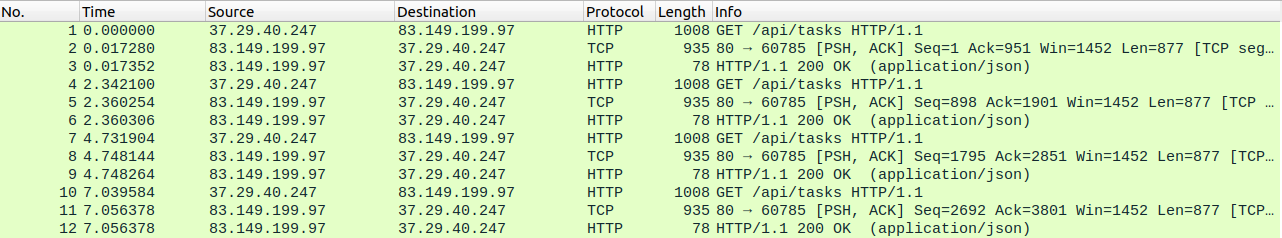
\includegraphics[width =\textwidth]{Wireshark.png}
        \caption{Пример работы Wireshark.}\label{wireshark}
    \end{center}
\end{figure}

В таблицах \ref{train_dataset} и \ref{test_dataset} представлены характеристики полученных данных для генерации сигнатур и их тестирования.
Классы протоколов дополнительно не балансировались.
В случае обучающего датасета нас интересуют потоки, содержащие хотя бы 5 пакетов, так как в слишком коротких потоках сигнатуры может не быть.
Для тестирования был добавлен дополнительный класс <<other>>, в который включены
все остальные не рассматриваемые протоколы, и к которому классификатор будет относить все потоки, которым не соответствует ни одна сигнатура.

\begin{table}[ht]
    \caption{Данные для генерации сигнатур.}
    \label{train_dataset}
    \centering
    \resizebox{0.9\columnwidth}{!}{
    \begin{tabular}{|c|c|c|c|c|c|c|}
        \hline
        Протокол   & \begin{tabular}[c]{@{}c@{}}Размер, \\ МБ\end{tabular} & \begin{tabular}[c]{@{}c@{}}Количество \\ пакетов\end{tabular} & \begin{tabular}[c]{@{}c@{}}Количество \\ потоков\end{tabular} &  \begin{tabular}[c]{@{}c@{}}Avg \\ bytes/pkt \end{tabular} &  \begin{tabular}[c]{@{}c@{}}Avg \\ pkts/stream \end{tabular} & \begin{tabular}[c]{@{}c@{}} Количеcтво \\ потоков: \\ $\geq$ 5 pkts \end{tabular} \\ \hline
        bittorrent & 272,4      & 240159             & 708                & 1134                             & 339                                 & 214                                          \\ \hline
        dns        & 130,7      & 1283082            & 204150             & 102                              & 6                                   & 11027                                        \\ \hline
        ftp        & 0,86       & 16959              & 735                & 51                               & 23                                  & 725                                          \\ \hline
        http       & 1811,5     & 799062             & 13710              & 2268                             & 58                                  & 1500                                         \\ \hline
        imap       & 22,0       & 27702              & 66                 & 793                              & 419                                 & 65                                           \\ \hline
        pop        & 0,06       & 919                & 59                 & 64                               & 16                                  & 40                                           \\ \hline
        smtp       & 13,5       & 59121              & 1120               & 229                              & 53                                  & 799                                          \\ \hline
    \end{tabular}}
\end{table}

\begin{table}[ht]
    \caption{Данные для тестирования сигнатур.}
    \label{test_dataset}
    \centering
    \resizebox{0.8\columnwidth}{!}{
    \begin{tabular}{|c|c|c|c|c|c|}
        \hline
        Протокол   & \begin{tabular}[c]{@{}c@{}}Размер, \\ МБ\end{tabular} & \begin{tabular}[c]{@{}c@{}}Количество \\ пакетов\end{tabular} & \begin{tabular}[c]{@{}c@{}}Количество \\ потоков\end{tabular} &  \begin{tabular}[c]{@{}c@{}}Avg \\ bytes/pkt \end{tabular} &  \begin{tabular}[c]{@{}c@{}}Avg \\ pkts/stream \end{tabular}\\ \hline
        bittorrent & 1,26       & 9409               & 876                & 133                              & 11                                  \\ \hline
        dns        & 53,3       & 664809             & 27800              & 80                               & 24                                  \\ \hline
        ftp        & 0,19       & 4000               & 294                & 48                               & 14                                  \\ \hline
        http       & 1494       & 406030             & 4607               & 3681                             & 88                                  \\ \hline
        imap       & 3,38       & 10587              & 143                & 320                              & 74                                  \\ \hline
        other      & 1119       & 1235122            & 18846              & 906                              & 66                                  \\ \hline
        pop        & 0,02       & 344                & 21                 & 58                               & 16                                  \\ \hline
        smtp       & 5,8        & 34428              & 1018               & 170                              & 34                                  \\ \hline
    \end{tabular}}
\end{table}

\subsection{Особенности при генерации сигнатур}

\begin{enumerate}
    \item
    Необходимо рассматривать только двунаправленные потоки, так как для генерации должны использоваться однородные потоки.
    Например, в случае HTTP набор общих подстрок для запрос и ответов разный.
    Поэтому необходимо либо уметь разделять потоки по направлениям и генерировать для каждого направления свою сигнатуру,
    либо не учитывать направление вовсе и генерировать общую сигнатуру.
    В первом случае, если не проводить семантический анализ протокола, то можно считать, что первый захваченный пакет
    в соединение идет от клиента к серверу, но это верно только для случая когда известно начало соединения.
    Это накладывает большое ограничение на выборку данных для генерации.
    Поэтому дальше будем рассматривать только двунаправленные потоки.

    \item
    Сигнатура обычно располагается в начале потока, поэтому не имеет смысла анализировать весь поток.
    Подбор константы первых анализируемых пакетов или байт полезной нагрузки является эвристическим.
    При этом привязку лучше делать по количеству пакетов из-за сильного разброса размеров пакетов разных протоколов,
    так как согласно \cite{park2008towards} сигнатура содержится в первых 10 пакетах потока.

    \item
    Необходимо ввести следующее эвристическое ограничение на сигнатуры, чтобы исключить тривиальные сигнатуры из рассмотрения:
    общая длина одной последовательности подстрок не меньше 8 символов
    и состоит хотя бы из 2 подстрок, каждая из которых не меньше 3 символов.

    \item
    Алгоритм AutoSig ввел дерево подстрок.
    Данная структура хороша тем, что увеличивает мощность получаемых сигнатур,
    это позволяет выделить несколько последовательностей подстрок, которые могут охватить те ситуация, в которых
    приложение имеет сильно разные потоки (например, поток управления и поток данных в FTP).
    Однако в том в виде, в котором это дерево представлено в работе \cite{ye2009autosig}, получается сильно избыточный результат.
    Если узел является сигнатурным и не листом, то по свойству этого узла его набор потоков является строгим надмножеством
    наборов потоков любых других сигнатурных узлов, находящихся в его поддереве (например, листы, которые всегда являются сигнатурными),
    таким образом, любые пути из сигнатурных узлов поддерева являются избыточными, так как если нашлась последовательность подстрок
    соответствующая сигнатурному узлу из рассматриваемого поддерева,
    то найдётся в потоке и последовательность подстрок, соответствующая рассматриваемому узлу.
    При этом специфичность нашей сигнатуры за счёт этих сигнатурных узлов не увеличивается,
    так как для совпадения со сигнатурой достаточно совпадения последовательности подстрок,
    соответствующей нашему узлу, которая уже включена в другие.
    А значит поддерево можно удалить. Однако если не выполняется строгость надмножества, то последовательности строк
    поддерева не будут включаться друг в друга, а полнота покрытия потоков сохраниться,
    при этом вырастит специфичность (чем длиннее последовательность подстрок, тем специфичнее сигнатура).
    Именно поэтому при таком условии узел не становится сигнатурным.
\end{enumerate}

\subsection{Выбор алгоритма для автоматической генерации сигнатур}

В таблице \ref{methods} проведен сравнительный анализ рассмотренных ранее методов

\begin{table}[ht]
    \caption{Сравнительный анализ методов автоматической генерации сигнатур.}
    \label{methods}
    \centering
    \resizebox{\columnwidth}{!}{
    \begin{tabular}{|c|c|c|c|}
        \hline
        Показатель\textbackslash{}Метод &
            LASER (LCS) &
            AutoSig &
            SigBox \\ \hline
        Тип сигнатуры &
            \begin{tabular}[c]{@{}c@{}}сигнатура пакета\\ (сигнатура потока)\end{tabular} &
            сигнатура потока &
            сигнатура потока \\ \hline
        Формат сигнатуры &
            \begin{tabular}[c]{@{}c@{}}последовательность \\ подстрок\end{tabular} &
            \begin{tabular}[c]{@{}c@{}}набор последовательностей \\ подстрок\end{tabular} &
            \begin{tabular}[c]{@{}c@{}}последовательность \\ подстрок\end{tabular} \\ \hline
        Тип ограничения &
            \begin{tabular}[c]{@{}c@{}}количество пакетов \\ (размер полезной нагрузки)\end{tabular} &
            размер полезной нагрузки &
            размер полезной нагрузки \\ \hline
        Агрегация потоков &
            не хранятся все потоки &
            хранятся все потоки &
            хранятся все потоки \\ \hline
        Параметр поддержки &
            отсутствует &
            присутствует &
            \begin{tabular}[c]{@{}c@{}}не является \\ параметром алгоритма\end{tabular} \\ \hline
        \end{tabular}}
\end{table}


\subsection{Реализация алгоритма LASER}



\newpage
